% !TEX root = top.tex
\section{Background}
We review the two major building blocks of our model: graph neural networks and hypernetworks.

\paragraph{Graph Neural Network:}
A graph neural network \citep{ScarselliGTHM09,li2015gated,KipfW16} is a collection of nodes and
edges $(\gV, \gE)$, where each node is a recurrent neural network (RNN) that individually sends and
receives messages along the edges, spanning over the horizon of message passing. Each node $v$
stores an internal node embedding vector $\vh_v^{(t)} \in \mathbb{R}^D$, and is updated recurrently:
\begin{equation}
\label{eq:gnn_prop}
\vh_v^{(t+1)} = 
\begin{cases}
U \left(\vh_v^{(t)}, \vm_v^{(t)} \right) \ \ & \text{if node $v$ is active},\\
\vh_v^{(t)} \ \ & \text{otherwise},
\end{cases}
\end{equation}
where $U$ is a recurrent cell function and $\vm_v^{(t)}$ is the message received by $v$ at time step
$t$:
\begin{equation}
\vm_v^{(t)}=\sum_{u\in N_{in}(v)} M \left(\vh_u^{(t)} \right),
\end{equation}
with $M$ the message function and $N_{in}(v)$ the set of neighbors with incoming edges
pointing towards $v$. $U$ is often modeled with a long short-term memory (LSTM) unit
\citep{hochreiter97lstm} or gated recurrent unit (GRU) \citep{cho14gru}, and $M$ with an MLP. Given
a graph $\gA$, we define the GNN operator $G_\gA$ to be a mapping from a set of initial node
embeddings $\{\vh_v^{(0)}\}$ to a set of different node embeddings $\{\vh_v^{(t)}\}$, parameterized by
some learnable parameters $\vphi$:
\begin{equation}
\left\{\vh_v^{(t)} | v \in \gV\right\} = 
G_\gA^{(t)} \left(\left\{\vh_v^{(0)} | v \in \gV \right\}; \vphi \right).
\end{equation}
Throughout propagation the node embeddings $\vh_v^{(t)}$ continuously aggregate graph level
information, which  can be used for tasks such as node prediction and   graph prediction by further
aggregation. Similar to RNNs, GNNs are typically learned using backpropagation through time (BPTT)
\citep{bptt}.

\paragraph{Hypernetwork:}
A hypernetwork \citep{ha2016hypernetworks} is a neural network that generates the parameters of
another network. For a typical deep feedforward network with $D$ layers, the parameters of the
$j$-th layer $W_j$ can be generated by a learned function $H$:
\begin{equation}
W_j = H(z_j), \ \ \forall j = 1, \dots, D,
\end{equation}
where $z_j$ is the layer embedding, and $H$ is shared for all layers. 
The output dimensionality of the hypernetwork is fixed, but it's possible to accommodate predicting weights for layers of varying kernel sizes by concatenating multiple kernels of the fixed size. Varying spatial sizes can also be accommodated by slicing in the spatial dimensions. Hypernetworks have been found effective in standard image recognition and text classification problems, and can be viewed as a relaxed weight sharing mechanism. Recently, they have shown to be effective in accelerating architecture search \citep{brock2017smash}.

\section{Graph Hypernetworks for Neural Architectural Search}
Our proposed Graph HyperNetwork (GHN) is a composition of a graph neural network and a hypernetwork.
It takes in a computation graph (CG) and generates all free parameters in the graph. During
evaluation, the generated parameters are used to evaluate the fitness of a random architecture, and
the top performer architecture on a separate validation set is then selected. This allows us to
search over a large number of architectures at the cost of training a single GHN. We refer the
reader to Figure~\ref{fig:main} for a high level system overview.

\begin{figure}
\vspace{-0.9cm}
\iflatexml
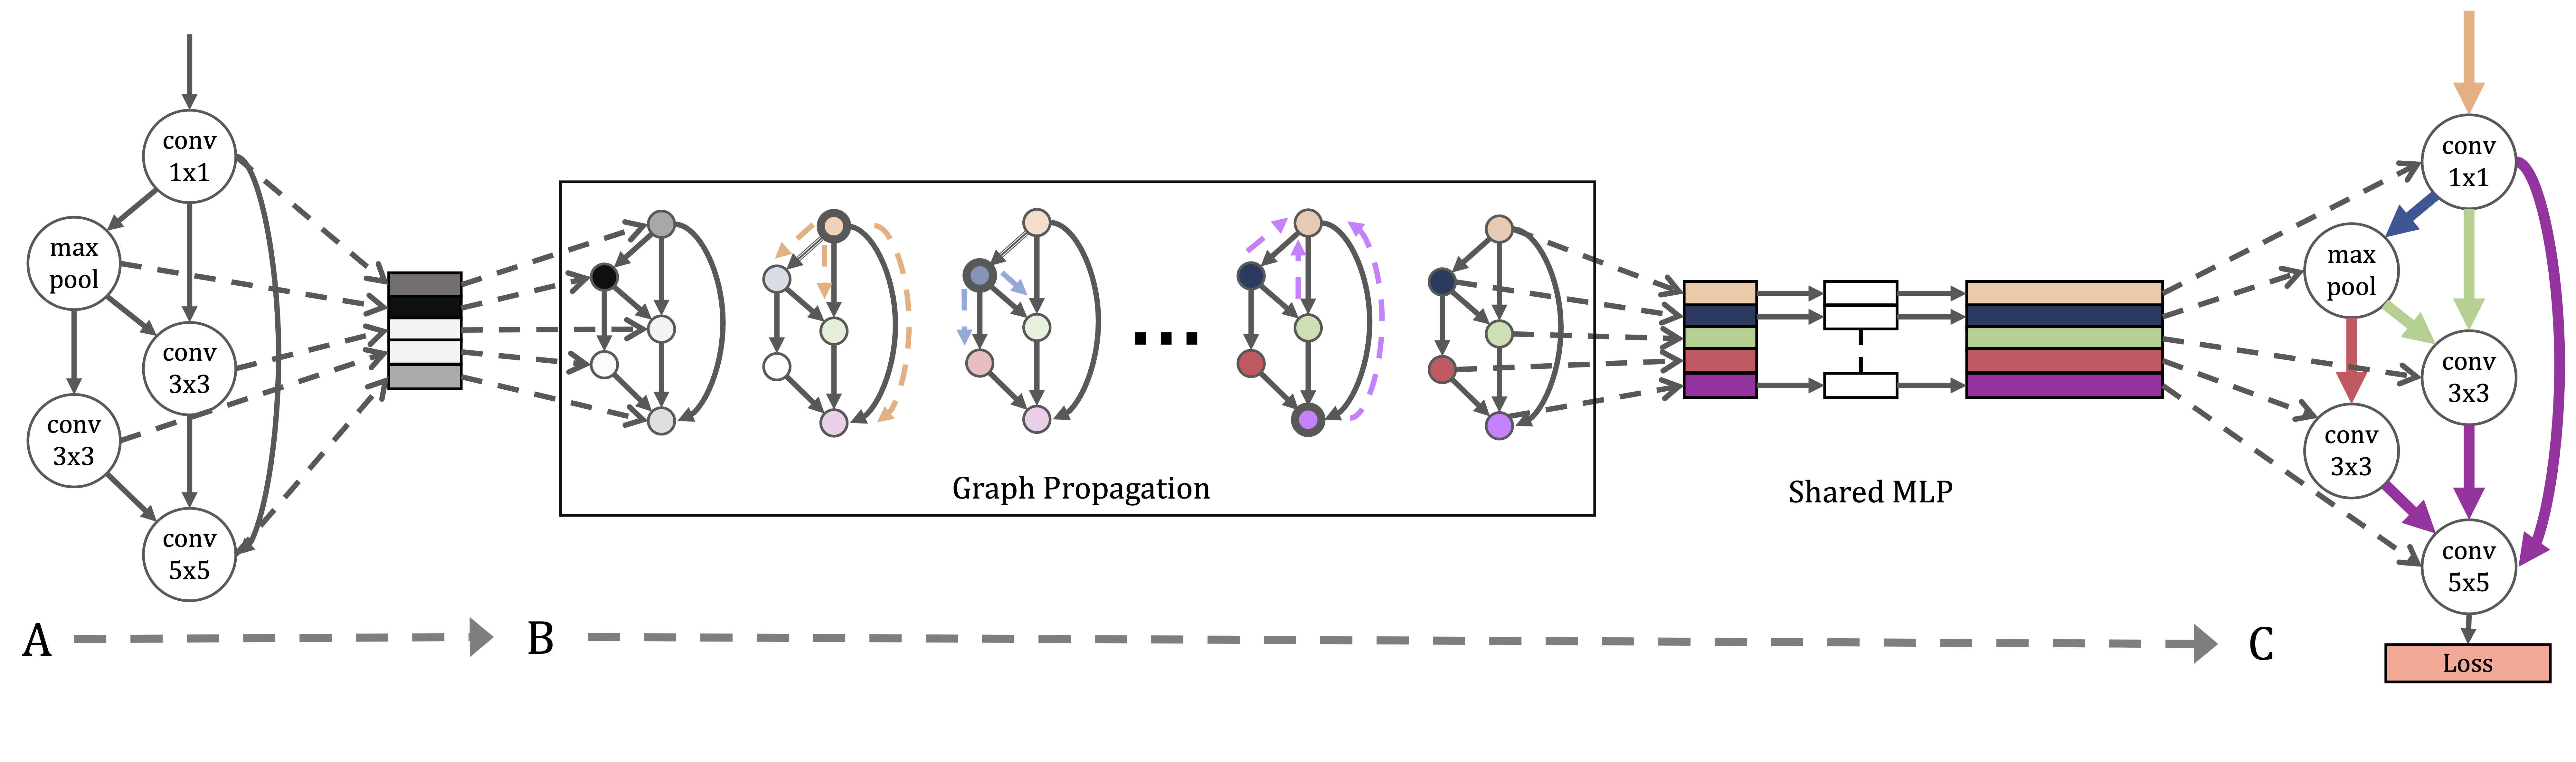
\includegraphics[width=6\linewidth]{figures/main3.png}
\else
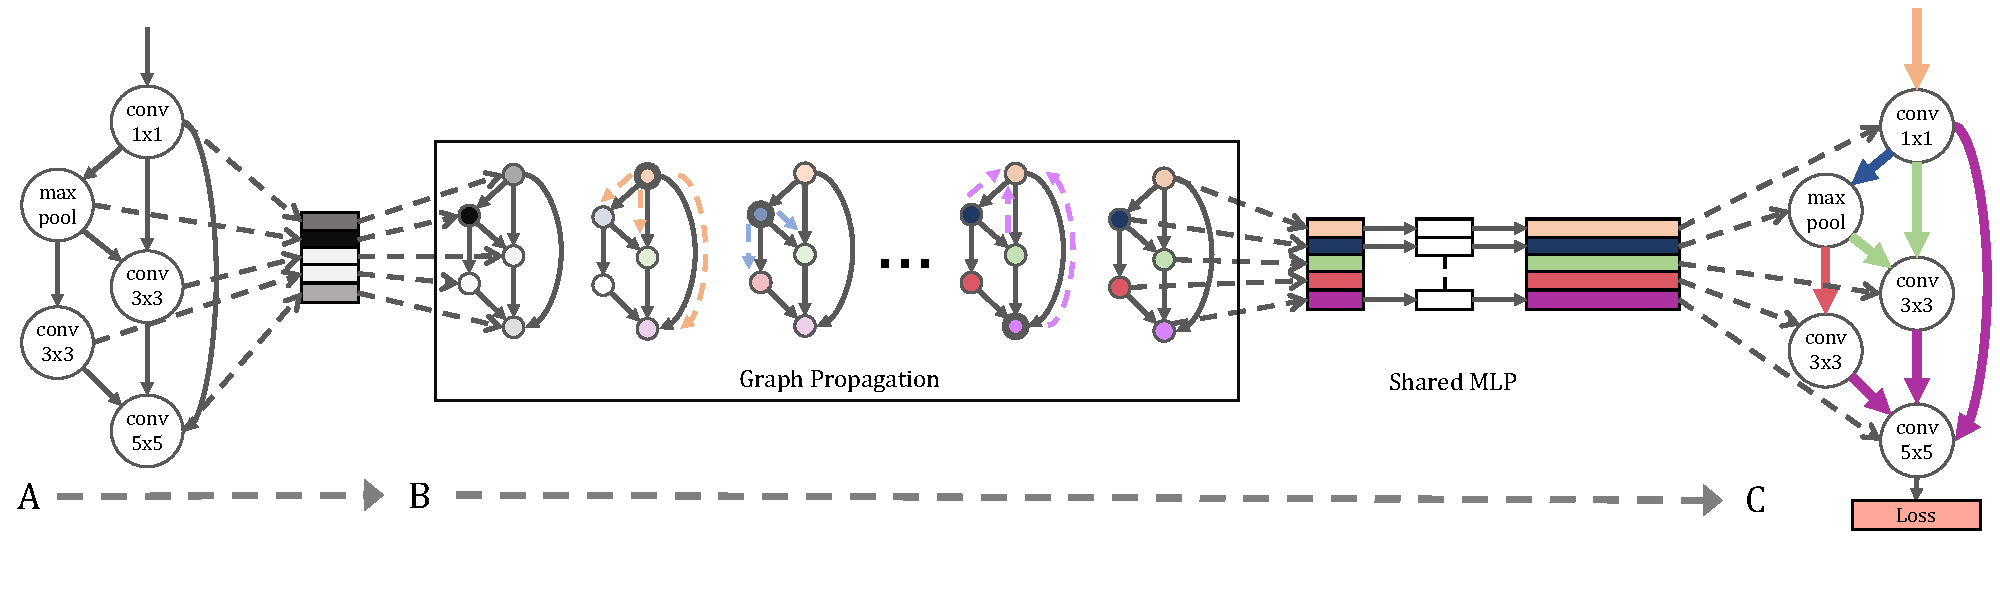
\includegraphics[width=\linewidth]{figures/main3.pdf}
\fi
\vspace{-1cm}
\caption{Our system diagram. \textbf{A}: A neural network architecture
is randomly sampled, forming a GHN. \textbf{B}: After graph propagation, each node in the GHN
generates its own weight parameters. \textbf{C}: The GHN is trained to minimize the training loss of
the sampled network with the generated weights. Random networks are ranked according to their
performance using GHN generated weights. }
\label{fig:main}
\vspace{-0.3cm}
\end{figure}

\subsection{Graphical Representation}
We represent a given architecture as a directed acyclic graph $\gA = (\gV, \gE)$, where each node $v
\in \gV$  has an associated computational operator $f_v$ parametrized by $w_v$, which produces an
output activation tensor $x_v$. Edges $e_{u \mapsto v} = (u, v) \in \gE$ represent the flow of
activation tensors from node $u$ to node $v$. $x_v$ is computed by applying its associated
computational operator on each of its inputs and taking summation as follows
\begin{equation}
\label{eq:compute_node}
x_v = \sum_{e_{u \mapsto v} \in \gE} f_v(x_u; w_v), \ \ \forall v \in \gV.
\end{equation}

\subsection{Graph Hypernetwork}
Our proposed Graph Hypernetwork is defined as a composition of a GNN and a hypernetwork. First,
given an input architecture, we used the graphical representation discussed above to form a graph
$\gA$. A parallel GNN $G_\gA$ is then constructed to be \textit{homomorphic} to $\gA$ with the exact
same topology. Node embeddings are initialized to one-hot vectors representing the node's
computational operator. After graph message-passing steps, a hypernet uses the node embeddings to
generate each node's associated parameters. Let $\vh_v^{(T)}$ be the embedding of node $v$ after $T$
steps of GNN propagation, and let $H \left(\cdot; \vvphi\right)$ be a hypernetwork parametrized by
$\vvphi$, the generated parameters $\tilde{\vw}_v$ are:
\begin{equation}
\tilde{\vw}_v = H \left(\vh_v^{(T)}; \vvphi\right).
\end{equation}
For simplicity, we implement $H$ with a multilayer perceptron (MLP). It is important to note that
$H$ is shared across all nodes, which can be viewed as an output prediction branch in each node of
the GNN. 
Thus the final set of generated weights of the entire architecture $\tilde{\vw}$ is found by applying $H$ on all the nodes and their respective embeddings which are computed by $G_\gA$:
\begin{align}
\tilde{\vw}=\left\{\tilde{\vw}_v | \ v \in \gV  \right\}
   &= \left\{H\left(\vh_v^{(T)}; \vvphi\right) \big| \ v \in \gV  \right\} \\
  &=  \left\{H\left(\vh; \vvphi\right) \big| \ \vh \in G_\gA^{(T)}\left(\left\{\vh_v^{(0)} \big| v \in \gV \right\}; \vphi\right)\right\} \\
  &= GHN\left(\gA; \vphi, \vvphi\right).
\end{align}

\subsection{Architectural Motifs and Stacked GNNs}
\label{section:graph_cells}

\iflatexml
\begin{figure}
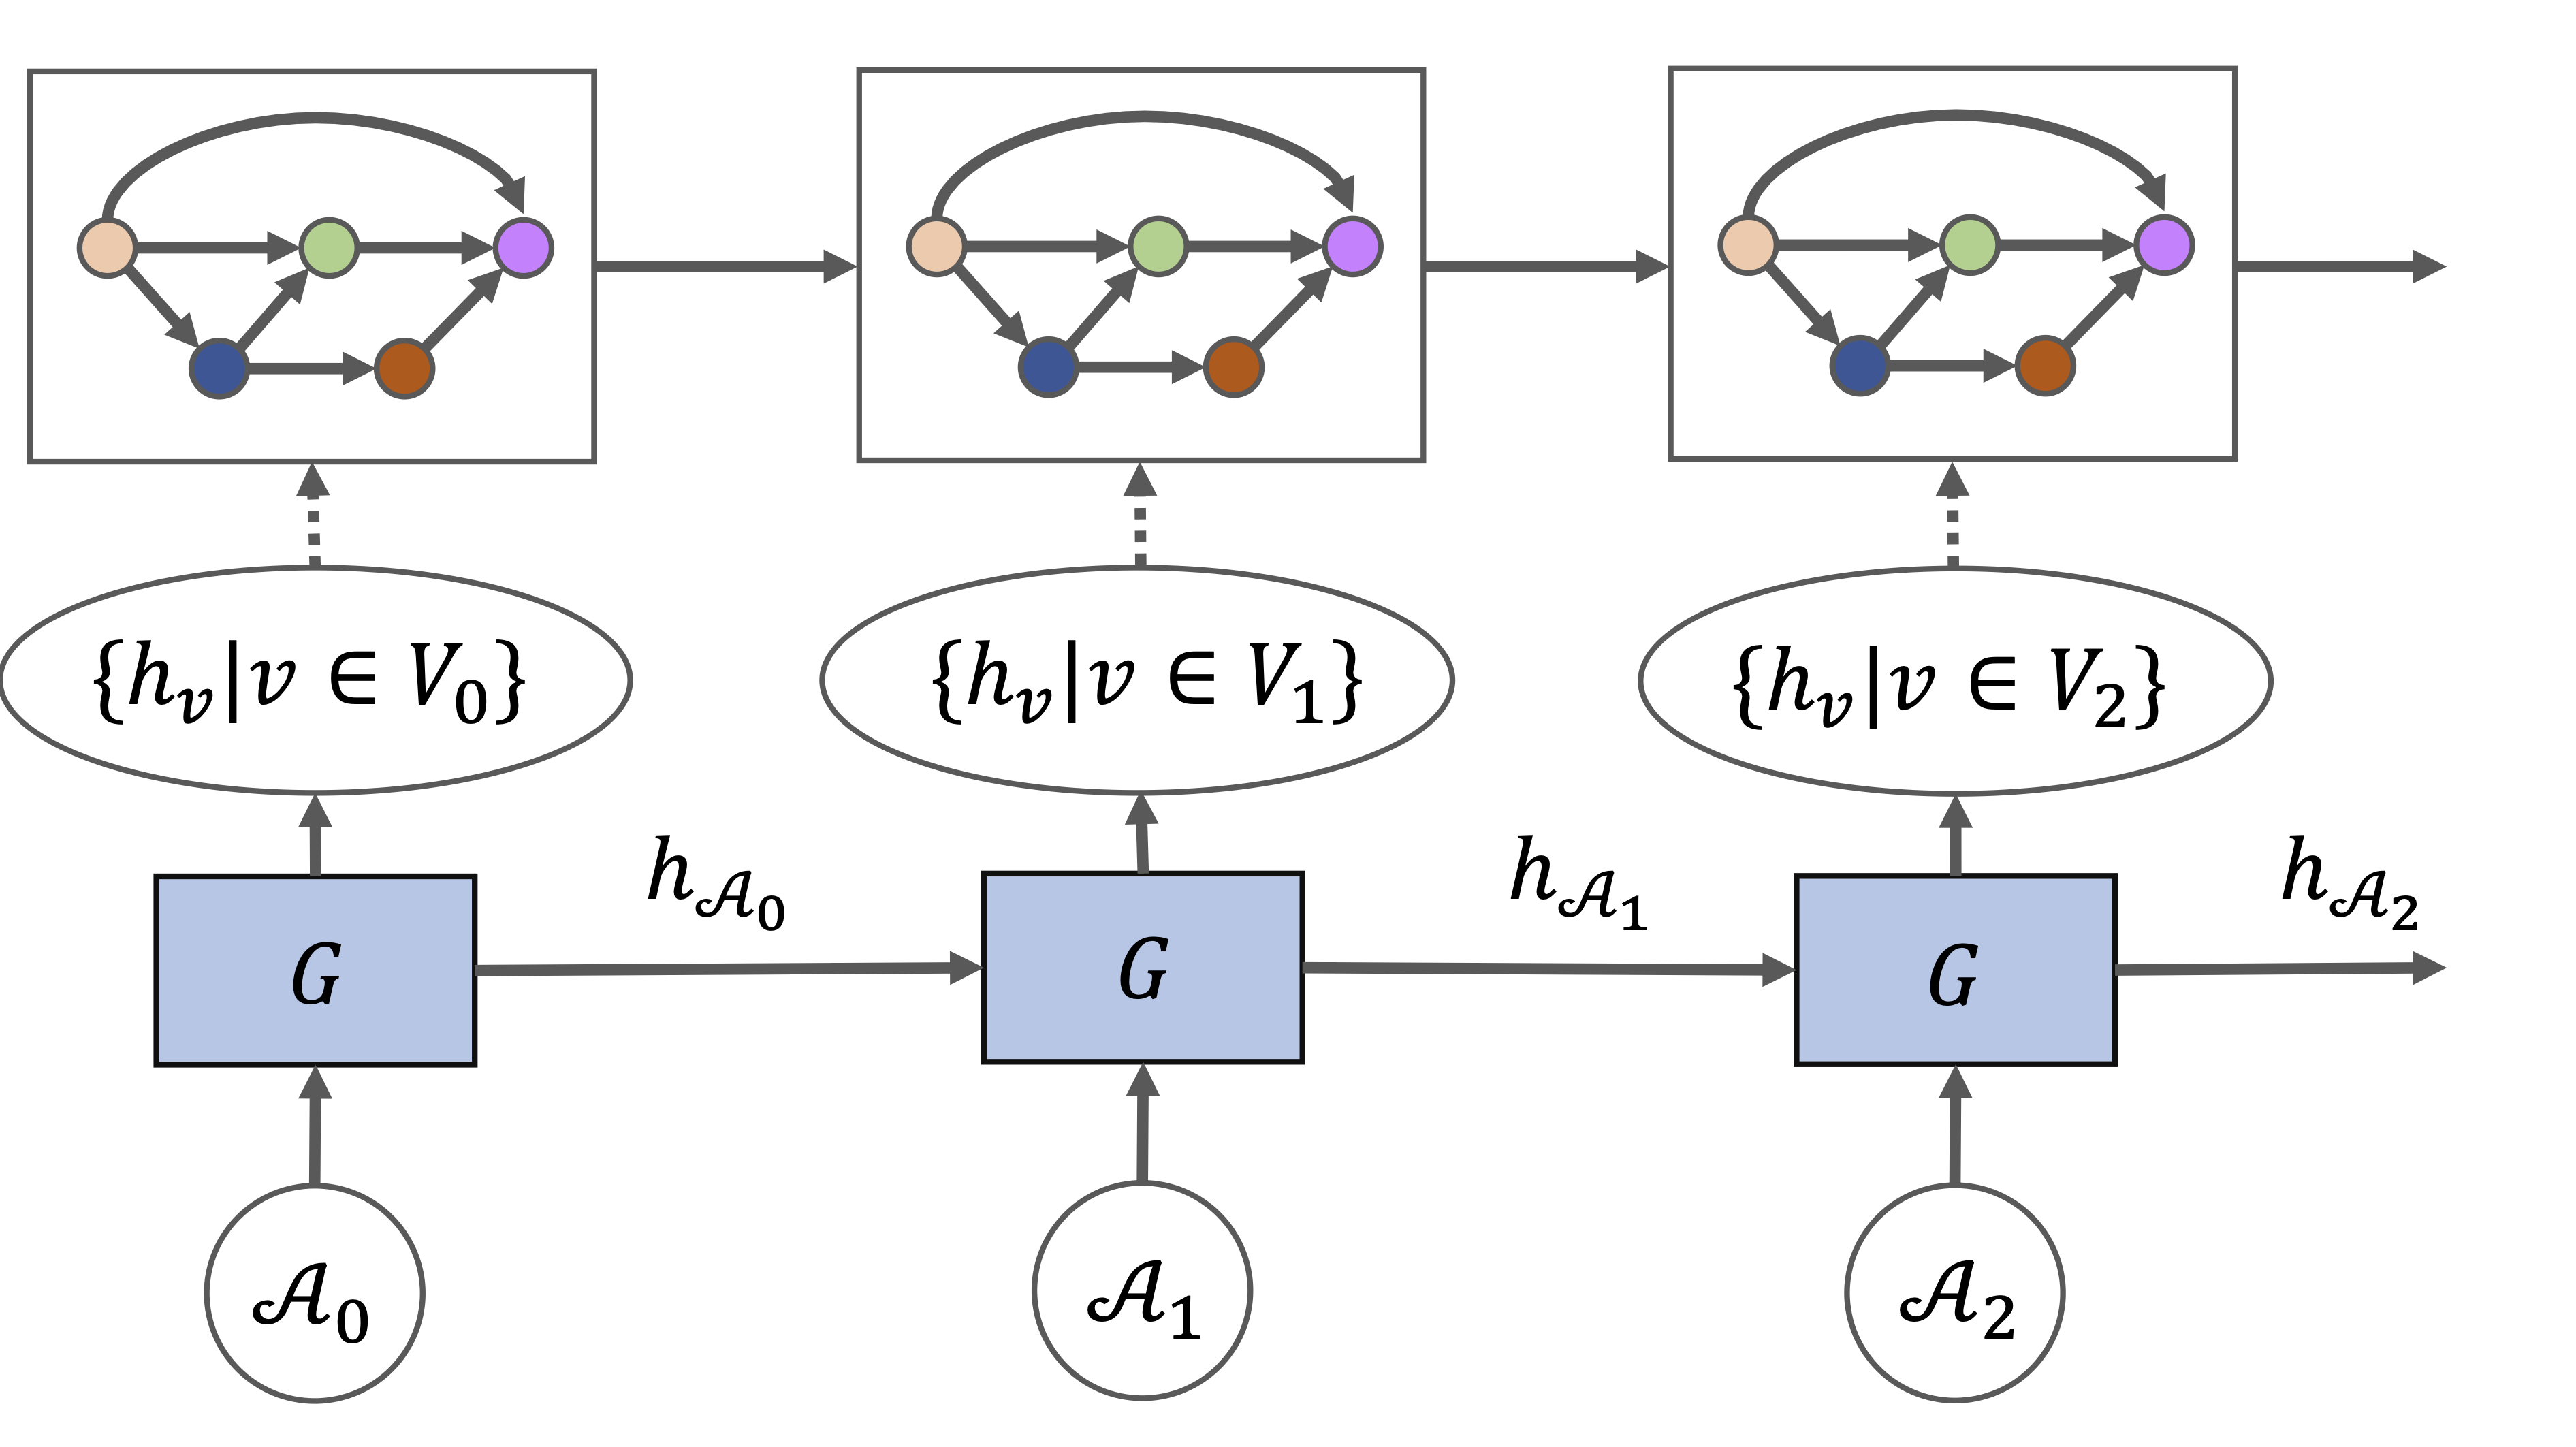
\includegraphics[width=4\linewidth]{figures/graph_cells.png}
\caption{Stacked GHN along the depth dimension.}
\label{fig:graph_cells}
\end{figure}
\else
\begin{wrapfigure}[]{r}{0.33\textwidth}
\vspace*{-0.5cm}
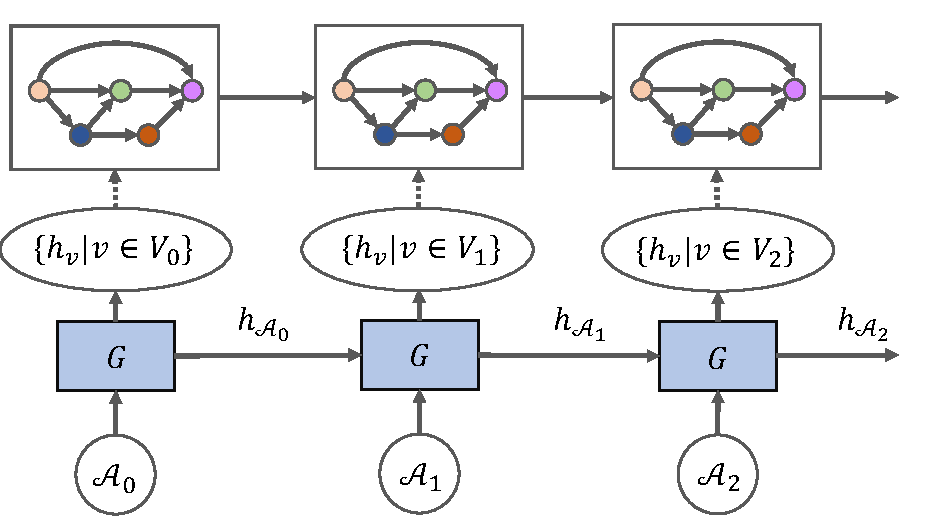
\includegraphics[width=\linewidth]{figures/graph_cells.pdf}
\caption{Stacked GHN along the depth dimension.}
\label{fig:graph_cells}
\end{wrapfigure}
\fi
The computation graph of some popular CNN architectures often spans over hundreds of nodes
\citep{he2016deep,huang2017densely}, which makes the search problem scale poorly. Repeated
architecture motifs are originally exploited in those architectures where the computation of each
computation block at different resolutions is the same, e.g. ResNet \citep{he2016resnet}. Recently,
the use of architectural motifs also became popular in the context of neural architecture search,
e.g. \citep{zoph2017learning, pham2018efficient}, where a small graph module with a fewer number of
computation nodes is searched, and the final architecture is formed by repeatedly stacking the same
module. \cite{zoph2017learning} showed that this leads to stronger performance due to a reduced
search space; the module can also be transferred to larger datasets by adopting a different
repeating pattern.

Our proposed method scales naturally with the design of repeated modules by stacking the same graph
hypernetwork along the depth dimension. Let $\gA$ be a graph composed of a chain of repeated modules
$\{\gA_i\}_{i=1}^N$. A graph level embedding $\vh_{\gA_i}$ is computed by taking an average over all
node embeddings after a full propagation of the current module, and passed onwards to the input node
of the next module as a message before graph propagation continues to the next module.
\begin{align}
\vh_{\gA_0} &= 0,\\
\vh_{\gA_i} &= \frac{1}{|\gV_i|}\sum_{v\in \gV_i} \left\{\vh_v^{(T)} | v \in \gV_i \right\} \label{eq:agg}\\
            &= \frac{1}{|\gV_i|}\sum G_{\gA_i}^{(T)}\left(\left\{\vh_v^{(0)} | v \in \gV_i \right\}, \vh_{\gA_{i-1}}; \vphi\right) \ \ \forall i > 0 \label{eq:next_cell}
\end{align}
Note that $G_{\gA_i}$ share parameters for all $\gA_i$.  Please see Figure~\ref{fig:graph_cells} for an overview.

\subsection{Forward-backward GNN message passing}
\label{sec:prop_scheme}
Standard GNNs employ the \textit{synchronous propagation scheme} \citep{li2015gated}, where the node
embeddings of all nodes are updated simultaneously at every step (see Equation~\ref{eq:gnn_prop}).
Recently, \cite{liao2018graph} found that such propagation scheme is inefficient in passing
long-range messages and suffers from the vanishing gradient problem as do regular RNNs. To mitigate
these shortcomings they proposed \textit{asynchronous propagation} using graph partitions. In our
application domain, deep neural architectures are chain-like graphs with a long diameter; This can
make synchronous message passing difficult. Inspired by the backpropagation algorithm, we propose
another variant of asynchronous propagation scheme, which we called \textit{forward-backward}
propagation, that directly mimics the order of node execution in a backpropagation algorithm.
Specifically, let $s$ be a topological sort of the nodes in the computation graph in a forward pass,
\begin{equation}
\label{eq:gnn_prop2}
\vh_v^{(t+1)} = 
\begin{cases}
U \left(\vh_v^{(t)}, \vm_v^{(t)} \right) \ \ & \text{if } s(t) = v \text{ and } 1 \le t \le |\gV|\\
  \ \ & \text{or if } s(2|\gV| - t) = v \text{ and } |\gV| + 1 \le t < 2|\gV|,\\
\vh_v^{(t)} \ \ & \text{otherwise}.
\end{cases}
\end{equation}
The total number of propagation steps $T$ for a full forward-backward pass will then become $2|\gV|-1$. Under the synchronous scheme,  propagating information across a graph with diameter $|\gV|$ would require $O(|\gV|^2)$ messages. This is reduced to $O(|\gV|)$ under the forward-backward scheme.

\subsection{Learning}
Learning a graph hypernetwork is straightforward since $\tilde{\vw}$ are directly generated by a
differentiable network. We compute gradients of the graph hypernetwork parameters $\vphi, \vvphi$
using the chain rule:
\begin{equation}
\nabla_{\vphi, \vvphi}{\gL_{train}(\tilde{\vw})} = \nabla_{\tilde{\vw}}{
\gL_{train}(\tilde{\vw})} \cdot \nabla_{\vphi, \vvphi}{\tilde{\vw}}
\end{equation}
The first term is the gradients of standard network parameters, the second term is decomposed as\begin{align}
 \nabla_\vphi{\tilde{\vw}} &= \left\{ \nabla_\vh H( \vh; \vvphi) \cdot \nabla_\vphi \vh \ \big| \ \vh \in G^{(T)} \left( \{\vh_v^{(0)}\}, \gA, \vphi \right) \right\}, \label{eq:gnn_grad}  \\ 
 \nabla_\vvphi{\tilde{\vw}} &= \left\{ \nabla_\vvphi H( \vh_v^{(T)}; \vvphi) \ \big| \ v \in \gV \right\} \label{eq:hypernet_grad}
\end{align}
where (Eq. \ref{eq:gnn_grad}) is the contribution from GNN module $G$ and (Eq.
\ref{eq:hypernet_grad}) is the contribution from the hypernet module $H$. Both $G$ and $H$ are
jointly learned throughout training.